\subsection{Direction Estimation}
\label{subsec:03_directionCandidates}

Delay samples are computed by the \ac{TDOA} methods introduced in the previous
sections.
Using \cref{eq:02_tdoaAngle}, one positive and one negative signed angle $\gamma'$
arise relative to the vector between the channels.
\Cref{fig:03_tdoaCode} is used to illustrate the terms and visualize the
circumstances for better understanding.
The definition of \textit{base channel} and \textit{next channel} stays as introduced
in \cref{subsec:03_microphones}.
Positive delay between two channels implies that a signal source
is closer to the base channel than the next channel.
For example if the detected delay has the same value as the maximum possible number
of samples between those channels, the source direction is equal to the
\textit{max-delay vector} in the figure.
In this case, $\gamma'$ is zero.
For all smaller delays greater than zero, two direction candidates \textit{candidate 0}
and \textit{candidate 1} result in the range of the max-delay vector $\pm \pi$.
The same applies mirrored for negative delays.
% -------------------------------------------------------------
\todo{ich würde auch an $\gamma'$ in der Figure noch die Richtung, weg vom max-delay vector definieren. Sonst ist das mit den anderen Pfeilen verwirrend. } \todo{the angle definiton of gamma is not the same as given in fig 3.1 but rather 90° minus gamma}
\begin{figure}[ht]
	\centering
		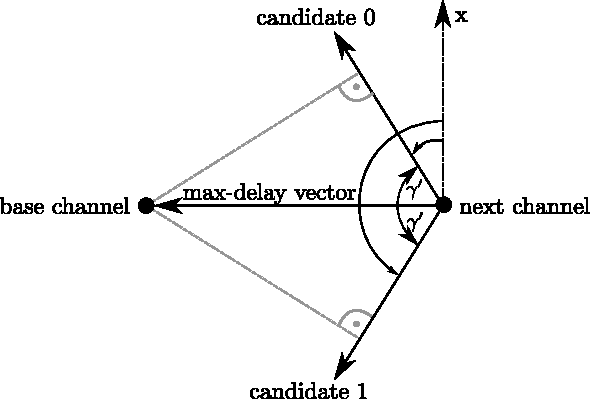
\includegraphics[width=0.6\columnwidth]{figures/tdoa_code}
	\caption{Illustration of the resulting candidates of \ac{TDOA} implementation.}
	\label{fig:03_tdoaCode}
\end{figure}

% -------------------------------------------------------------

By this implementation, all candidates are represented in the robot coordinate system.
Having four channels, each neighboring channel pair returns two candidate directions.
Diagonal channels can be paired as well for the correlation methods.
However, this case is not considered profoundly in this work due to the overdetermined
system by four pairs.
Out of these eight candidates, a final direction angle $\gamma$ is chosen
by computing all combinations and selecting the one with smallest sum of angle difference \todo{differences? Vielleicht hier einmal als Formel aufschreiben?}.
During research, different factors like signal strength \todo{zweites Beispiel wenn vorhanden} were tested to include
more a priori knowledge.
Due to lack of reliability, no additional signal properties are taken into account.

There exists one exceptional case, where the signal source is detected straight in front
or behind the robot and distance can be estimated.
If this is the case, the direction angle is corrected to 0 or $\pi$.
How the distance information is handled is content of the next section.
